\documentclass[14pt]{extbook}
\usepackage{multicol, enumerate, enumitem, hyperref, color, soul, setspace, parskip, fancyhdr} %General Packages
\usepackage{amssymb, amsthm, amsmath, bbm, latexsym, units, mathtools} %Math Packages
\everymath{\displaystyle} %All math in Display Style
% Packages with additional options
\usepackage[headsep=0.5cm,headheight=12pt, left=1 in,right= 1 in,top= 1 in,bottom= 1 in]{geometry}
\usepackage[usenames,dvipsnames]{xcolor}
\usepackage{dashrule}  % Package to use the command below to create lines between items
\newcommand{\litem}[1]{\item#1\hspace*{-1cm}\rule{\textwidth}{0.4pt}}
\pagestyle{fancy}
\lhead{Makeup Progress Quiz -1}
\chead{}
\rhead{Version C}
\lfoot{7547-2949}
\cfoot{}
\rfoot{Fall 2020}
\begin{document}

\begin{enumerate}
\litem{
Describe the end behavior of the polynomial below.\[ f(x) = 9(x + 2)^{4}(x - 2)^{9}(x - 9)^{3}(x + 9)^{5} \]\begin{enumerate}[label=\Alph*.]
\begin{multicols}{2}\item 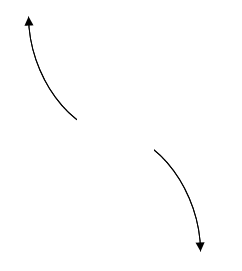
\includegraphics[width = 0.3\textwidth]{../Figures/polyEndBehaviorAC.png}\item 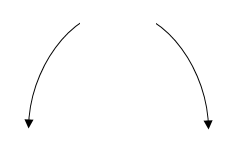
\includegraphics[width = 0.3\textwidth]{../Figures/polyEndBehaviorBC.png}\item 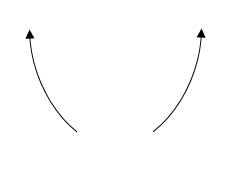
\includegraphics[width = 0.3\textwidth]{../Figures/polyEndBehaviorCC.png}\item 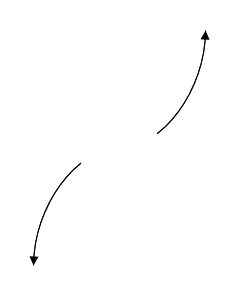
\includegraphics[width = 0.3\textwidth]{../Figures/polyEndBehaviorDC.png}\end{multicols}\item None of the above.
\end{enumerate} }
\litem{
Describe the zero behavior of the zero $x = 8$ of the polynomial below.\[ f(x) = 8(x + 8)^{7}(x - 8)^{12}(x - 4)^{4}(x + 4)^{8} \]\begin{enumerate}[label=\Alph*.]
\begin{multicols}{2}\item 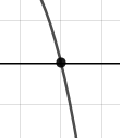
\includegraphics[width = 0.3\textwidth]{../Figures/polyZeroBehaviorCopyAC.png}\item 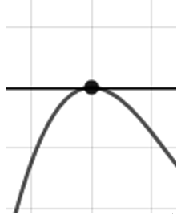
\includegraphics[width = 0.3\textwidth]{../Figures/polyZeroBehaviorCopyBC.png}\item 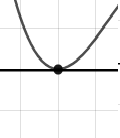
\includegraphics[width = 0.3\textwidth]{../Figures/polyZeroBehaviorCopyCC.png}\item 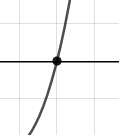
\includegraphics[width = 0.3\textwidth]{../Figures/polyZeroBehaviorCopyDC.png}\end{multicols}\item None of the above.
\end{enumerate} }
\litem{
Construct the lowest-degree polynomial given the zeros below. Then, choose the intervals that contain the coefficients of the polynomial in the form $x^3+bx^2+cx+d$.\[ -4 + 2 i \text{ and } 1 \]\begin{enumerate}[label=\Alph*.]
\item \( b \in [5, 17], c \in [12, 13], \text{ and } d \in [-24, -17] \)
\item \( b \in [-6, 2], c \in [-2, 6], \text{ and } d \in [-5, -2] \)
\item \( b \in [-13, -1], c \in [12, 13], \text{ and } d \in [19, 24] \)
\item \( b \in [-6, 2], c \in [-4, 0], \text{ and } d \in [-1, 7] \)
\item \( \text{None of the above.} \)

\end{enumerate} }
\litem{
Describe the zero behavior of the zero $x = -5$ of the polynomial below.\[ f(x) = 6(x + 4)^{12}(x - 4)^{9}(x - 5)^{5}(x + 5)^{2} \]\begin{enumerate}[label=\Alph*.]
\begin{multicols}{2}\item 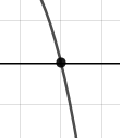
\includegraphics[width = 0.3\textwidth]{../Figures/polyZeroBehaviorAC.png}\item 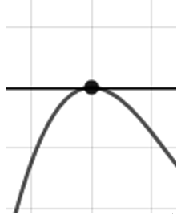
\includegraphics[width = 0.3\textwidth]{../Figures/polyZeroBehaviorBC.png}\item 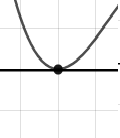
\includegraphics[width = 0.3\textwidth]{../Figures/polyZeroBehaviorCC.png}\item 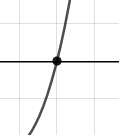
\includegraphics[width = 0.3\textwidth]{../Figures/polyZeroBehaviorDC.png}\end{multicols}\item None of the above.
\end{enumerate} }
\litem{
Which of the following equations \textit{could} be of the graph presented below?
\begin{center}
    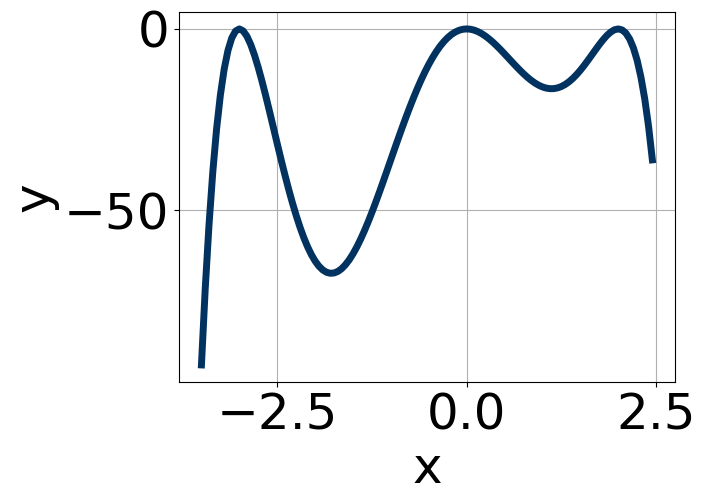
\includegraphics[width=0.5\textwidth]{../Figures/polyGraphToFunctionCopyC.png}
\end{center}
\begin{enumerate}[label=\Alph*.]
\item \( 16x^{10} (x + 3)^{10} (x - 2)^{5} \)
\item \( -8x^{9} (x + 3)^{8} (x - 2)^{5} \)
\item \( -19x^{4} (x + 3)^{10} (x - 2)^{11} \)
\item \( 5x^{10} (x + 3)^{10} (x - 2)^{4} \)
\item \( -12x^{6} (x + 3)^{6} (x - 2)^{10} \)

\end{enumerate} }
\litem{
Which of the following equations \textit{could} be of the graph presented below?
\begin{center}
    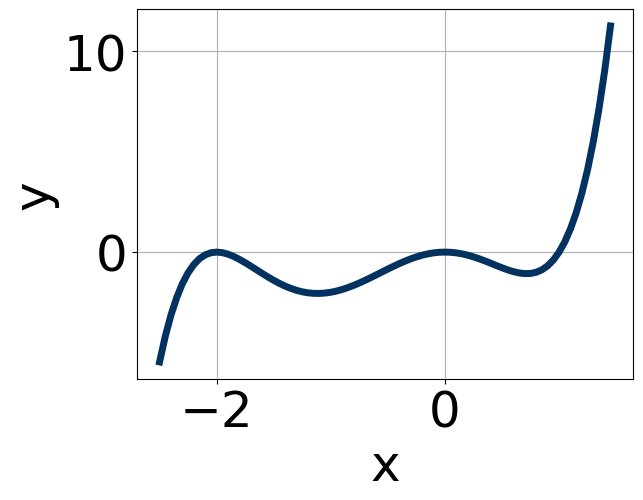
\includegraphics[width=0.5\textwidth]{../Figures/polyGraphToFunctionC.png}
\end{center}
\begin{enumerate}[label=\Alph*.]
\item \( 2x^{4} (x + 2)^{6} (x - 1)^{7} \)
\item \( -20x^{6} (x + 2)^{8} (x - 1)^{7} \)
\item \( -20x^{10} (x + 2)^{6} (x - 1)^{4} \)
\item \( 9x^{5} (x + 2)^{8} (x - 1)^{9} \)
\item \( 14x^{5} (x + 2)^{4} (x - 1)^{8} \)

\end{enumerate} }
\litem{
Describe the end behavior of the polynomial below.\[ f(x) = -8(x + 8)^{5}(x - 8)^{6}(x - 2)^{2}(x + 2)^{3} \]\begin{enumerate}[label=\Alph*.]
\begin{multicols}{2}\item 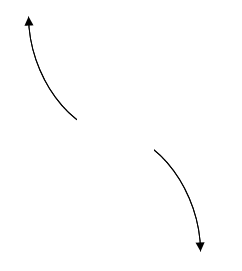
\includegraphics[width = 0.3\textwidth]{../Figures/polyEndBehaviorCopyAC.png}\item 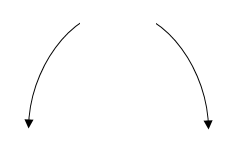
\includegraphics[width = 0.3\textwidth]{../Figures/polyEndBehaviorCopyBC.png}\item 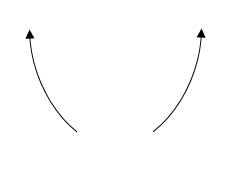
\includegraphics[width = 0.3\textwidth]{../Figures/polyEndBehaviorCopyCC.png}\item 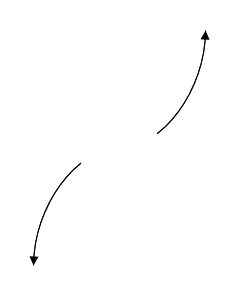
\includegraphics[width = 0.3\textwidth]{../Figures/polyEndBehaviorCopyDC.png}\end{multicols}\item None of the above.
\end{enumerate} }
\litem{
Construct the lowest-degree polynomial given the zeros below. Then, choose the intervals that contain the coefficients of the polynomial in the form $ax^3+bx^2+cx+d$.\[ \frac{2}{5}, \frac{1}{5}, \text{ and } 5 \]\begin{enumerate}[label=\Alph*.]
\item \( a \in [20, 28], b \in [-140, -132], c \in [71, 78], \text{ and } d \in [-17, -9] \)
\item \( a \in [20, 28], b \in [-111, -108], c \in [-73, -71], \text{ and } d \in [-17, -9] \)
\item \( a \in [20, 28], b \in [-140, -132], c \in [71, 78], \text{ and } d \in [3, 13] \)
\item \( a \in [20, 28], b \in [137, 143], c \in [71, 78], \text{ and } d \in [3, 13] \)
\item \( a \in [20, 28], b \in [-120, -116], c \in [-29, -19], \text{ and } d \in [3, 13] \)

\end{enumerate} }
\litem{
Construct the lowest-degree polynomial given the zeros below. Then, choose the intervals that contain the coefficients of the polynomial in the form $x^3+bx^2+cx+d$.\[ -5 + 5 i \text{ and } -2 \]\begin{enumerate}[label=\Alph*.]
\item \( b \in [4, 22], c \in [68, 74], \text{ and } d \in [92, 107] \)
\item \( b \in [-1, 10], c \in [2, 12], \text{ and } d \in [9, 19] \)
\item \( b \in [-1, 10], c \in [-3, -1], \text{ and } d \in [-13, -9] \)
\item \( b \in [-13, -3], c \in [68, 74], \text{ and } d \in [-102, -96] \)
\item \( \text{None of the above.} \)

\end{enumerate} }
\litem{
Construct the lowest-degree polynomial given the zeros below. Then, choose the intervals that contain the coefficients of the polynomial in the form $ax^3+bx^2+cx+d$.\[ \frac{3}{4}, -4, \text{ and } \frac{-2}{3} \]\begin{enumerate}[label=\Alph*.]
\item \( a \in [10, 16], b \in [-35, -30], c \in [-67, -55], \text{ and } d \in [-26, -22] \)
\item \( a \in [10, 16], b \in [41, 52], c \in [-10, -6], \text{ and } d \in [24, 25] \)
\item \( a \in [10, 16], b \in [-48, -40], c \in [-10, -6], \text{ and } d \in [24, 25] \)
\item \( a \in [10, 16], b \in [64, 69], c \in [72, 82], \text{ and } d \in [24, 25] \)
\item \( a \in [10, 16], b \in [41, 52], c \in [-10, -6], \text{ and } d \in [-26, -22] \)

\end{enumerate} }
\end{enumerate}

\end{document}